\documentclass{article}
\usepackage{graphicx}
\usepackage[margin=0.7in]{geometry}
\usepackage{amsmath} % For mathematical typesetting

\title{Devoir libre}
\author{Mohammed Khatiri - CPI1}

\begin{document}
\maketitle

\begin{center}
    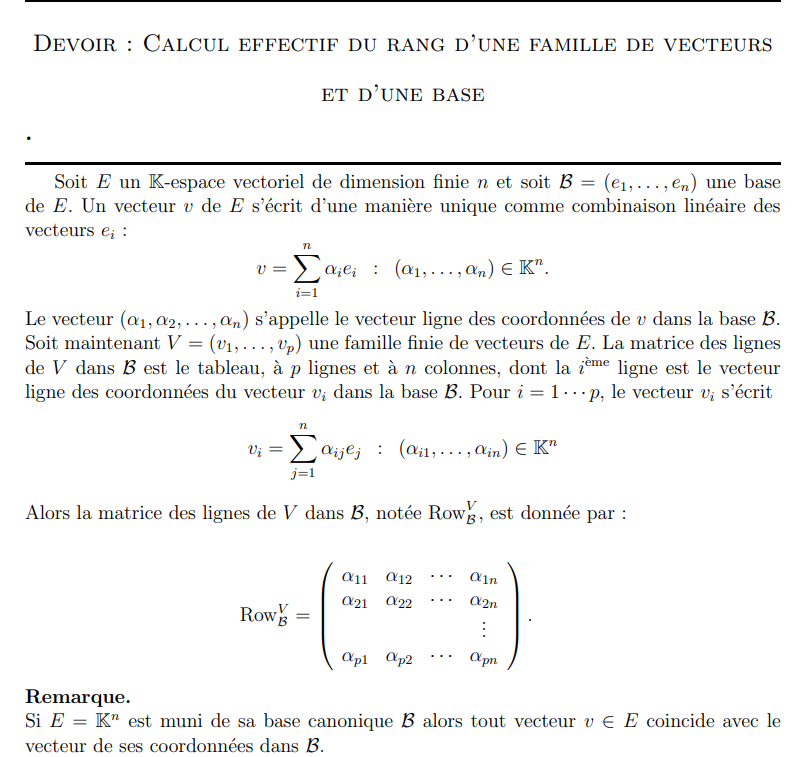
\includegraphics[scale=0.7]{exo.png}
\end{center}

\newpage

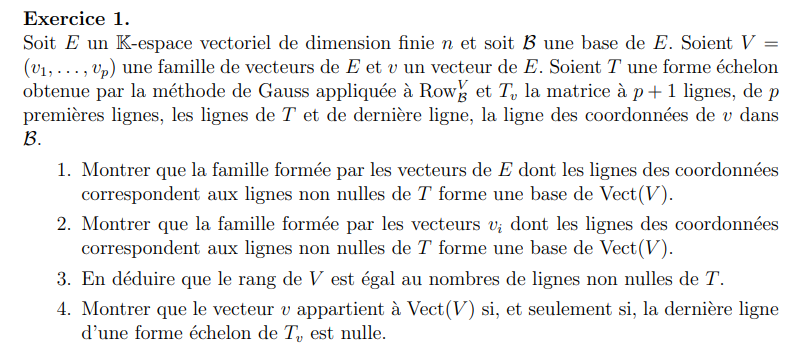
\includegraphics[scale=1]{questions.png}

\section*{Réponses:}
\section*{1.}
Prenons $v$ un vecteur de la famille $\text{Vect}(V)$, il s'écrit sous la forme : $\sum_{i=1}^{n}\alpha_{i}v_{i}$.
Chaque vecteur des lignes de $T$: $(u_i \in E/i \in (1,...,p))$, s'écrivent sous la forme: $u_i = \sum_{j=i}^{p}\beta_{j,i}v_j$, pour tout $\beta_{j,i} \neq 0$. Puisque chaque ligne de la matrice en forme échelonée est une combinaison linéaire des lignes initiales précédentes de la matrice, on peut montrer que les vecteurs $v_i$ sont des combinaisons linéaires des vecteurs $u_i$.\newline
on a: pour i = p: $u_p = \beta_{p,p}v_p$ donc $\exists\gamma_{p,p}\in{K}: v_p = \gamma_{p,p}u_p$.\newline
supposant que :$\forall i \in{p,p-1,...,n} :\forall{v_i}\in{V}:\exists{(\gamma_{i,j}\in K/j\in(p,p-1,p-2,...,i))} : v_i = \sum_{j=i}^{p}\gamma_{j,i}u_j$.\newline
montrons que c'est vrai pour n+1;\newline
on a: $u_{n+1}=\sum_{j=n+1}^{p}\beta_{j,n+1}v_j$, donc $u_{n+1} = \sum_{j=n}^{p}\beta_{j,n+1}v_j + \beta_{n+1,n+1}v_{n+1} = \sum_{j=n}^{p}\beta_{j,n+1}\sum_{k=j}^{p}\gamma_{k,j}u_k + \beta v_{n+1}$.\newline
bien que:\newline
$\exists{(\gamma_{k,n+1}\in{K}/k\in{p,p-1,...,n})} : \sum_{j=n}^{p}\frac{\beta_{j,n+1}}{\beta}\sum_{k=j}^{p}\gamma_{k,j}u_k  = \sum_{k=n}^{p}\gamma_{k,n+1}u_k$.\newline
donc: $\frac{1}{\beta}u_{n+1} - \sum_{k=n}^{p}\gamma_{k,n+1}u_k = v_{n+1}$.\newline
donc même n+1 vérifie;\newline
d'où tout $v_i$ est une combinaison linéaire de vecteur $u_i$, d'où la famille $K = (u_i)$ est génératrice de Vect(V), de méme la famille $B = (u_i/u_i \neq 0) = (w_i)$ est génératrice de cardinal p'.\newline\newline

supposant mainetenant que cette famille B est liée:\newline
d'où: $\exists{w_k},\alpha_j: w_k = \sum_{j=1}^{k-1} \alpha_jw_j +\sum_{j=k+1}^{p'} \alpha_jw_j$.\newline
bien que d'aprés la matrice obtenue: on a: \newline
$\forall{w_i}\in{E},\exists{!l_i\in\mathbf N},\exists!(\delta_j\in{K}): w_i = \sum_{j=l_i}^{n}\delta_j e_j$ telle que la suite $(l_i)$ est décroissante et $\delta_{l_i}\neq 0$ .\newline
or $\exists!(\delta'_j\in{K}) : \sum_{j=1}^{k-1} \alpha_j w_j = \sum_{j=l}^{n}\delta'_je_j$ où $l>l_k$ et $\delta'_{l} \neq 0$ si $\alpha_j \neq 0,\forall j<k$.\newline
,$\exists!(\delta'_j\in{K}) : \sum_{k+1}^{p'} \alpha_j w_j = \sum_{j=l'}^{n}\delta'_je_j$ où $l'<l_k$ et $\delta'_{l'} \neq 0$ si $\alpha_j \neq 0,\forall j>k$.\newline
;absurde; $w_k \neq \sum_{j=l}^{n}\delta''_je_j$ d'où $\alpha_j = 0,\forall j<k$.\newline
;de même; $w_k \neq \sum_{j=l'}^{n}\delta''_je_j$  puisque $\delta_{l_i}\neq 0$ :  d'où $\alpha_j = 0,\forall j>k$.\newline\newline

donc la famille B n'est pas liée. et d'où c'est une base de Vect(V).

\section*{2.}

\section*{3.}
Puisque $p'$ est le nombre de vecteurs non nuls formés par les lignes non nulles, on peut donc conclure que le cardinal de $B$ est le nombre de lignes non nulles, c'est-à-dire $p'$. Ainsi, $\text{Dim}(\text{Vect}(V)) = \text{Card}(B) = p'$. Par conséquent, le rang de $V$ est égal au nombre de lignes non nulles de $T$.
et d'où Dim(Vect(V)) = Card(B) = p'. d'où le rang de V est égale au nombres de lignes non nulles de T.

\section*{4.}


si $v \in Vect(V)$ alors: v s'ecrit comme combinaison linéaire des autre lignes de la matrice $T_v$.\newline
et d'où la forme échelonée de la matrice $T_v$ rendera la dernière ligne nulle.\newline
de même: si la dernière ligne de la matrice $T_v$ est nulle d'où: $\exists\alpha_i : v - \sum\alpha_iw_i = 0$.\newline
d'où: v est combinaison linéaire des $w_i$, d'où : $v \in Vect(V)$.



\end{document}